\chapter{Einleitung}
\section{Warum?}
Im zunehmenden Maße finden sich mobile Endgeräte (z.B. Tablet) als Marketing, Informations- und Imageelement, aber auch als Teil von Prozessen im Retail- als auch im Industrieumfeld wieder. Diese ersetzen oder erweitern bestehende Lösungen (z.b. Kiosk, Digital-Signage, Laptops, Industrie PCs) um interaktive Elemente und unterstützen so Unternehmen in ihren Geschäftsprozessen. 
Bei der eingesetzten Lösung ist es aus Sicht des Retail und Industrie-Kunden wichtig die Handhabung und das Erlebnis des Gerätes für den Anwender zu erhalten. Die Einsatzgebiete reichen dabei von Tablets in Produktionsprozessen zu Zwecken der Qualitätssicherung (eigene Applikationen mit Dokumentationsfunktionen) bis hin zu Multimedia-Terminals im stationären Handel. Um diese verschiedenen Szenarien realisieren zu können ist es notwendig eine stabile, sichere und wartbare Plattform zu konstruieren, die zum einen die Anwendung in unterschiedlichen Einsatzgebieten ermöglicht und zum anderen für den Betriebsführer leicht bereitzustellen und zu warten ist.\cite{lastenheft}
%Zitat fragwürdig?!
\paragraph*{}
Um den hier angeführten allgemeinen Anforderungen ihrer Kunden gerecht zu werden, benötigt Kapsch die passendste Softwarelösung im Bereich Security für die hierfür in Betracht gezogenen Tablets. Um diese Softwarelösung zu ermitteln, wurde ein Projektteam des fünften Jahrgangs der HTBLVA Spengergasse, Fachbereich Informatik mit der Aufgabe der Eruierung dieser Lösung und  der Erstellung eines Konzepts betraut. Das Projekt KTI – Kapsch Tablet Infrastructure wird von dem Projektmanager Philip Steinhäuser geleitet  und besteht aus den Teammitgliedern Sebastian Götze, Samuel Hammer, Kaufmann Michael und Konstanze Müller. Das Projektteam steht in engem Kontakt mit dem Project-owner welcher mit den Mitarbeitern Bernhard Bruckner und Jürgen Krammer vertreten ist. 
\paragraph*{}
Kapsch unterstützt das Projekt mit diversen Hilfeleistungen sowie Technischer Support, Intellektuelle Hilfe und finanzielle Unterstützung beim Kauf des Tablets, welches nach Beendigung des Projekts wieder in den Besitz von Kapsch übergehen wird.


\section{Ursprungsproblem}
Die Aufgabe von Kapsch an das Projektteam ist es, verschiedene Softwarelösungen zum Systemschutz von Android-Tablets zu testen. Die vom Projektowner zum Test gewünschten Softwarelösungen sind.
\begin{itemize}
	\item MDM
	\item MDM + Container
	\item Samsung Knox
\end{itemize}
Zusätzlich bestünde noch die Möglichkeit einer \textbf {Linux Manipulation}, welche jedoch für Kapsch aus rechtlichen Gründen nicht in Frage kommt, da diverse Garantieverletzungen auftreten würden und zusätzlich enorme Kosten anfallen würden aufgrund von Hohen Entwicklungskosten und langen Entwicklungszeiten bis das System einwandfrei funktionieren würde.
\paragraph*{}
Zu diesen Schutzsystemmöglichkeiten soll ein Untersuchungsbericht angefertigt werden. In diesem werden die Ergebnisse  festgehalten und verglichen, um das beste System für die Kunden von Kapsch zu ermitteln.
\paragraph*{}
Auf Basis dieses Untersuchungsberichts soll dann die Passendste Softwarelösung ausgewählt werden, welche in ein Konzept eingebaut wird. Ein Teil dieses Konzepts beinhaltet die Implementierung der ausgewählten Softwarelösung auf ein Tablet welches dann als Prototyp deklariert wird. 
\paragraph*{}
Der Untersuchungsbericht in Kombination mit dem Prototyp ist das Ergebnis was über den Ausgang dieses Projekts entscheidet.


\section{Vorgehensweise}
\subsection{Vorbereitung}
\begin{itemize}
	\item Vorbereitungsmeeting mit Kapsch
	\item Einlesen in Technologie
	\item Erste Recherchen
\end{itemize}
\subsection{Planung}
\begin{itemize}
	\item Projektantrag
	\item Vorstudie
	\item PSP (Projektstrukturplan)
	\item OSP (Objektstrukturplan)
	\item Timetable bzw. Gantt-Chart
	\item Lastenheft
	\item Pflichtenheft
	\item Projekthandbuch
	\item Checklist Template
	\item Research Template
	\item Untersuchungsbericht
	\item Diplomarbeit
\end{itemize}
\subsection{Durchführung}
\begin{itemize}
	\item Recherche
	\item Erstellung des Untersuchungsberichtes
	\item Auswahl der passenden Lösung
	\item Konzept erstellen
	\item Ausgewählte Lösung in Konzept einarbeiten
	\item Konzept teilweise umsetzen
	\begin{itemize}
		\item Konfiguration der Lösung auf Tablet (Prototyp
	\end{itemize}
\end{itemize}
\subsection{Ergebnis}
\begin{enumerate}
	\item Untersuchungsbericht
	\item Prototyp
\end{enumerate}

\subsection{Organigramm}
\begin{figure}[H]
	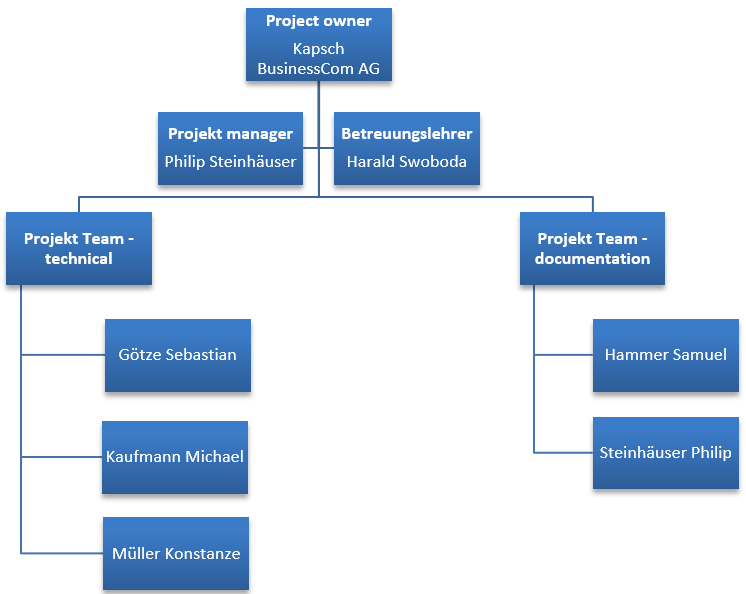
\includegraphics[scale=0.6]{Images/organigramm}
	\caption{Projekt-Organigramm}
\end{figure}
Die Aufgaben des Projekts wurden ab diesem Zeitpunkt so verteilt das das Dokumentationsteam sämtliche Projektmanagementaufgaben und das Technik Team alle Research- und Testungsaufgaben übernimmt.
\begin{figure}[H]
	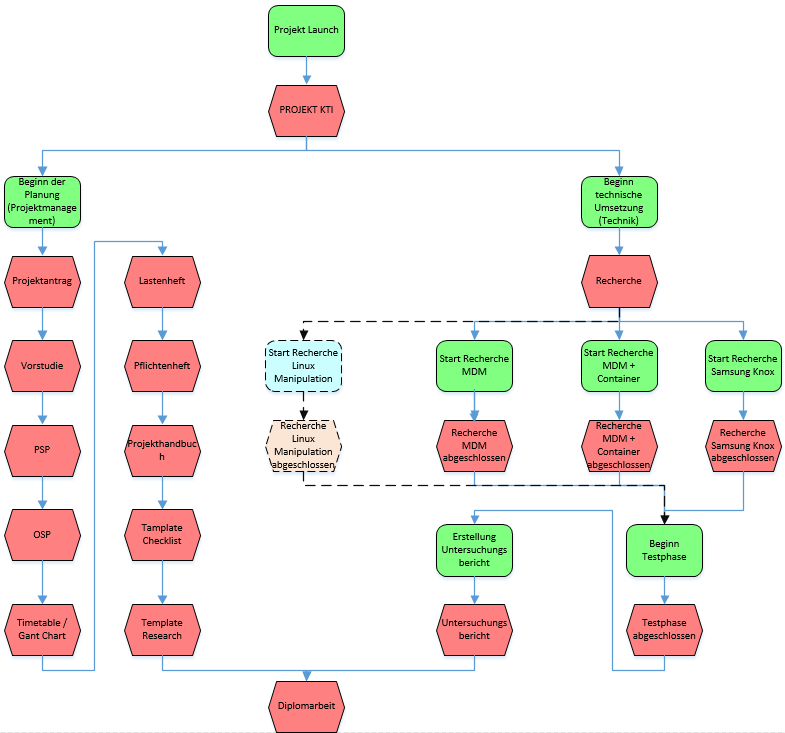
\includegraphics[scale=0.7]{Images/arbeitsteilung}
	\caption{Aufgabenverteilung - Diagramm}
\end{figure}
Diese Visio Grafik zeigt auf der einen Seite die Reihenfolge der erstellten Dokumente, so wie beispielsweise, dass der OSP und der Timetable / Gant Chart auf dem PSP aufbaut, da dieser zuvor erstellt wurde und diese drei Dokumente konsistent sein müssen.
\paragraph*{}
Auf der Technik Seite wiederum sieht man das zuerst eine umfangreiche Recherche nötig ist bzw. war, bevor die Wahl der passendsten Softwarelösung getroffen werden kann / konnte, welche dann schlussendlich für das Konzept und in weiterer Folge für die Konfiguration des Prototyps verwendet werden konnte / wurde.
\paragraph*{}
Wenn man sich unsere Vorgehensweise nun Schritt für Schritt auf die beiden Sub Teams aufgeteilt anschauen würde, würde folgendes Bild entstehen:

%\begin{center}
%    \begin{tabular}{| l | l | l |}
%    \hline
%    	1 & 
%     \\ \hline
%     \\ \hline
%     \\ \hline
%     \\ \hline
%    \end{tabular}
%\end{center}




	